\documentclass[11pt]{article}
\usepackage[margin=1in]{geometry}
\usepackage{amsmath}
\usepackage{amssymb}
\usepackage{amsthm}
\usepackage{booktabs}
\usepackage{xcolor}
\usepackage{graphicx}

\theoremstyle{definition}
\newtheorem{definition}{Definition}
\theoremstyle{plain}
\newtheorem{proposition}{Proposition}
\theoremstyle{remark}
\newtheorem{remark}{Remark}

\title{Input-oriented FDH Slack Analysis: \\ Formulation and Aggregate Decomposition}
\author{slackshare package (v0.1.0)}
\date{\today}

\begin{document}

\maketitle

\begin{abstract}
We formalize the input-oriented Free Disposal Hull (FDH) slack analysis used by the \texttt{slackshare} package (v0.1.0).
We define FDH-efficient input levels, compute avoidable slack per decision-making unit (DMU), and identify the peer
unit that sets the efficiency frontier for each DMU. We decompose total input across all DMUs into a system-wide ``slack share''
and per-DMU contributions. We then extend this analysis to panel data (multiple dates and input types) by analyzing independent
cross-sectional slices. The panel extension gracefully handles incomplete data: missing inputs or outputs for individual DMUs are
treated as ineligible for analysis at that slice, with results propagated as NA, while aggregate metrics are computed over the
observed (eligible) subset using skip-NA semantics. We formalize a catalogue of degenerate cases and their handling. Worked examples
illustrate the method on synthetic data and explore the curse of dimensionality in multi-output settings.
\end{abstract}

\section{Introduction: Visual Overview}

The following figures illustrate the key outputs of an FDH slack analysis on a synthetic panel dataset:

\begin{figure}[h]
\centering
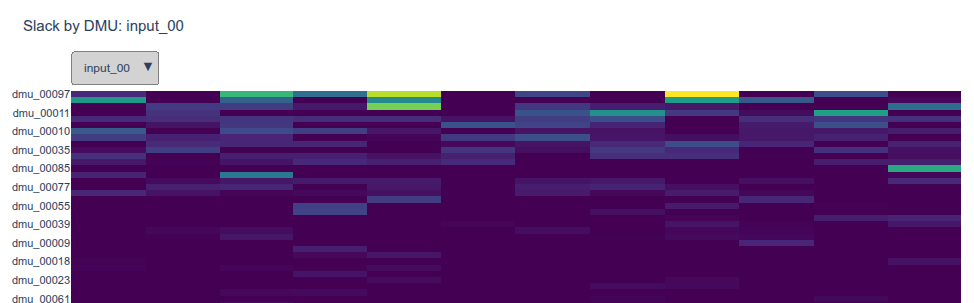
\includegraphics[width=0.85\textwidth]{../demo1.png}
\caption{\textbf{Slack by DMU (heatmap).} Each row is a decision-making unit; color intensity represents avoidable input slack over 12 monthly dates (purple = efficient, yellow = wasteful). DMUs are sorted by median slack, and a dropdown selector allows switching between all 40 input types. Hovering on a cell reveals the exact DMU, date, slack value, and the peer DMU that set the efficiency benchmark.}
\label{fig:slack_heatmap}
\end{figure}

\begin{figure}[h]
\centering
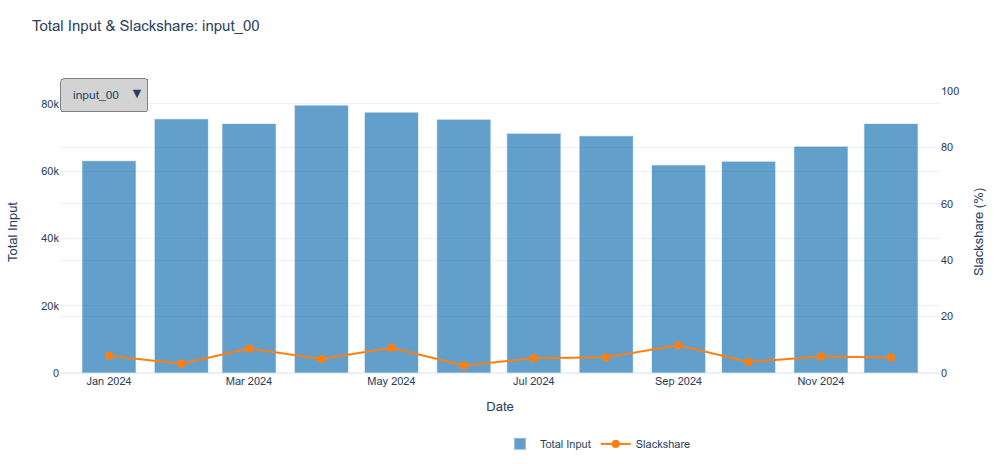
\includegraphics[width=0.85\textwidth]{../demo2.png}
\caption{\textbf{Total Input \& Slack Share (bar + line).} Blue bars show the population's aggregate input consumption over time. The orange line overlays the \emph{slack share} — the percentage of total input that is avoidable excess (waste). This metric reveals whether the population is becoming more or less efficient across the time horizon.}
\label{fig:slack_share}
\end{figure}

We now formalize the method that produces these figures.

\section{Setup and Notation}

Consider a set of $n$ decision-making units (DMUs), indexed $i = 1, \ldots, n$.
Each DMU $i$ consumes a single (typically undesirable) input $x_i \ge 0$ and produces a vector of $K$ outputs
$y_i = (y_i^1, \ldots, y_i^K) \in \mathbb{R}_{\ge 0}^K$.
Throughout, we write vector inequalities component-wise: $y_j \ge y_i$ means $y_j^k \ge y_i^k$ for all $k = 1, \ldots, K$.

\subsection*{Notation to Implementation}

The following table maps mathematical notation to \texttt{slackshare} function signatures and output columns:

\begin{table}[h]
\centering
\begin{tabular}{lll}
\toprule
\textbf{Concept} & \textbf{Notation} & \textbf{Code} \\
\midrule
DMU identifier & $i$ & \texttt{id\_col} parameter \\
DMU input value & $x_i$ & \texttt{input\_col} parameter \\
DMU output vector & $y_i$ & \texttt{output\_cols} parameter \\
Efficient input level & $x_i^*$ & \texttt{x\_star} column \\
Avoidable slack & $\text{slack}_i$ & \texttt{slack} column \\
Efficiency flag & $\text{slack}_i = 0$ & \texttt{efficient} column \\
Peer DMU (benchmark) & peer of $i$ & \texttt{peer} column \\
Slack share fraction & $\text{slack\_share}$ & summary dict key \\
\bottomrule
\end{tabular}
\end{table}

The package always computes the \texttt{peer} column, which identifies the benchmark unit (the one achieving $x_i^*$).
When multiple units tie for the minimum input among dominators, the alphabetically first DMU identifier breaks the tie.

\section{FDH Dominance and Efficient Input}

\begin{definition}[Dominance set]
The dominance set (or dominating set) of DMU $i$ is
\[ D(i) = \{ j \in \{1, \ldots, n\} : y_j \ge y_i \}. \]
By reflexivity, $i \in D(i)$ for all $i$.
\end{definition}

The efficient input level for DMU $i$ is the minimum input among all dominating units:
\begin{equation}
x_i^{*} = \min_{j \in D(i)} x_j.
\end{equation}

Since $i \in D(i)$, we have $x_i^* \le x_i$ always, and $x_i^*$ is well-defined and non-negative (even when $D(i) = \{i\}$ alone).
Hence, the slack $\text{slack}_i := x_i - x_i^* \ge 0$ is well-defined and non-negative.

\section{Slack and Efficiency}

The slack $\text{slack}_i = x_i - x_i^*$ represents the amount by which DMU $i$ could reduce its input while maintaining at least the same output performance (by replicating any unit in $D(i)$).

A DMU is \emph{FDH-efficient} if and only if $\text{slack}_i = 0$, i.e., $x_i = x_i^*$.
Equivalently, a DMU is efficient if it achieves the minimum input among all units that dominate it on every output.

\begin{remark}
FDH (Free Disposal Hull, \cite{DeprinsSimarTulkens1984}) imposes only free disposability and allows no convexity.
Thus, each DMU is only compared against \emph{actually observed} dominating units, never against hypothetical convex blends.
This contrasts with DEA (Data Envelopment Analysis, \cite{CharnesCooperRhodes1978}), which constructs a convex frontier and can benchmark against infeasible synthetic units.
For a given dataset, FDH yields a coarser (higher) frontier than DEA.
\end{remark}

\section{Aggregate Decomposition}

Define the total input and total slack as
\begin{align}
X &= \sum_{i=1}^{n} x_i, \\
S &= \sum_{i=1}^{n} \text{slack}_i.
\end{align}

The \emph{aggregate slack share} measures the fraction of total input across all DMUs that is avoidable excess:
\begin{equation}
\text{slack\_share} = \frac{S}{X}.
\end{equation}

Per-DMU contributions to the system are captured by two share metrics:
\begin{align}
\text{share\_of\_total\_input}_i &= \frac{\text{slack}_i}{X}, \\
\text{share\_of\_total\_slack}_i &= \begin{cases} \frac{\text{slack}_i}{S} & \text{if } S > 0, \\ 0 & \text{if } S = 0. \end{cases}
\end{align}

The first metric expresses each DMU's slack as a fraction of the population's total input.
The second expresses each DMU's waste as a fraction of system-wide waste (when any exists).
When $S > 0$, $\sum_{i=1}^{n} \text{share\_of\_total\_slack}_i = 1$ by definition of shares summing to one.

\section{Validity Conditions}

The analysis is well-defined and yields meaningful results under the following preconditions:

\begin{enumerate}
\item Each $x_i \ge 0$. (For slices/datasets with $X = \sum_i x_i = 0$, the ratio $\text{slack\_share} = S / X$ is undefined and a \texttt{ZeroDivisionError} is raised.)
\item For each $i$, the output vector $y_i$ is not identically zero: $\exists k \, y_i^k > 0$.
  (If $y_i \equiv 0$, then $D(i) = \{1, \ldots, n\}$ — the entire population trivially dominates $i$ — making $i$'s benchmark the single globally-cheapest DMU, unrelated to $i$'s actual profile. The package rejects all-zero-output rows to avoid this degenerate case.)
\item The dataset is non-empty: $n \ge 1$.
\end{enumerate}

\section{Worked Numerical Example}

\label{sec:example}

Consider a toy dataset with $n = 4$ DMUs, a single undesirable input (e.g., emissions), and one output (e.g., revenue):

\begin{table}[h]
\centering
\begin{tabular}{ccc}
\toprule
DMU & Input $x_i$ & Output $y_i$ \\
\midrule
A & 100 & 10 \\
B & 80 & 10 \\
C & 120 & 15 \\
D & 60 & 8 \\
\bottomrule
\end{tabular}
\end{table}

Compute the dominance set for each DMU:

\begin{itemize}
\item $D(A) = \{j : y_j \ge 10\} = \{A, B, C\}$ (A, B, and C all produce $\ge 10$). Thus $x_A^* = \min(100, 80, 120) = 80$.
\item $D(B) = \{j : y_j \ge 10\} = \{A, B, C\}$. Thus $x_B^* = \min(100, 80, 120) = 80$.
\item $D(C) = \{j : y_j \ge 15\} = \{C\}$ (only C produces $\ge 15$). Thus $x_C^* = 120$.
\item $D(D) = \{j : y_j \ge 8\} = \{A, B, C, D\}$ (all produce $\ge 8$). Thus $x_D^* = \min(100, 80, 120, 60) = 60$.
\end{itemize}

Compute slack and efficiency:

\begin{table}[h]
\centering
\begin{tabular}{ccccc}
\toprule
DMU & $x_i$ & $x_i^*$ & $\text{slack}_i$ & Efficient? \\
\midrule
A & 100 & 80 & 20 & No \\
B & 80 & 80 & 0 & Yes \\
C & 120 & 120 & 0 & Yes \\
D & 60 & 60 & 0 & Yes \\
\midrule
Total & 360 & 340 & 20 & --- \\
\bottomrule
\end{tabular}
\end{table}

Here, DMUs B, C, and D are efficient; only A is inefficient with slack of 20 units.
The system-wide slack share is $S / X = 20 / 360 = 0.0556$ (about 5.6\% of total input is avoidable).

\section{Computational Complexity}

For each slice (date, input type), the FDH computation involves:
\begin{itemize}
\item For each DMU $i$, identify the dominance set $D(i) = \{j : y_j \ge y_i \text{ on all } K \text{ dimensions}\}$ by scanning all $n$ units.
\item For each $i$, find $x_i^* = \min_{j \in D(i)} x_j$ among the dominators.
\end{itemize}
This yields $O(n^2)$ per-slice time complexity, since each of the $n$ DMUs requires a full $O(n)$ scan of dominance.
For datasets with many slices (dates $\times$ input types), the total cost can scale substantially; the per-slice loop is embarrassingly parallel
and can be sped up via \texttt{multiprocessing.Pool} to distribute slices across CPU cores.

\subsection*{Curse of Dimensionality}

A critical limitation of FDH (and DEA) in high output dimensions is the sharply rising fraction of ``trivially efficient'' DMUs.
As the number of output dimensions $K$ increases, the output space becomes sparse, and most units have unique output profiles undominated by any other.

To illustrate, we generated random single-input, $K$-output datasets with $n=100$ DMUs and uniformly random outputs in $[0, 10]$:

\begin{table}[h]
\centering
\begin{tabular}{ccc}
\toprule
$K$ (output dimensions) & \# Efficient DMUs & \% Efficient \\
\midrule
1 & 5 & 5.0\% \\
2 & 8 & 8.0\% \\
4 & 51 & 51.0\% \\
8 & 87 & 87.0\% \\
12 & 99 & 99.0\% \\
\bottomrule
\end{tabular}
\end{table}

This phenomenon suggests FDH analysis yields the most interpretable results in settings with a small to moderate number of outputs ($K \le 4$) and large sample sizes.
High-dimensional output spaces require either larger $n$ or dimensionality reduction (aggregation, PCA) to maintain discriminative power.

\section{Panel Data Analysis}

When data are panel-structured (multiple dates and/or input types), the analysis extends naturally:
we analyze independent cross-sectional slices, applying the single-input FDH method to each $(date, input\_type)$ pair.

\subsection{Balanced Panel (Current Implementation)}

For each date $t = 1, \ldots, T$ and input type $k = 1, \ldots, K_{\text{in}}$,
let $x_i^{(t,k)}$ denote the input value for DMU $i$ at date $t$ for input type $k$,
and let $y_i^{(t)}$ denote the (shared) output vector for DMU $i$ at date $t$
(outputs are typically not indexed by input type; the choice of input type does not change the set of achievable outputs in a given date).

In the balanced case, every $(dmu, date, input\_type)$ and $(dmu, date, output\_type)$ combination is required to be observed.
For the slice $(t, k)$, define the dominance set as
\[ D_{t,k}(i) = \{ j : y_j^{(t)} \ge y_i^{(t)} \}, \]
and the efficient input as
\[ x_{i,t,k}^{*} = \min_{j \in D_{t,k}(i)} x_j^{(t,k)}. \]

The slack, efficiency flag, and aggregate metrics follow as in \S\ref{sec:example}.
Crucially, analysis of slice $(t, k)$ is \emph{independent} of all other slices:
there is no pooling across dates or input types in the FDH frontier.

\subsection{Unbalanced Panel (Implemented)}

In practice, panel data are often incomplete: a DMU may not report a given input type, may have begun or ceased operations, or may have missing output values for structural reasons. We now formalize the unbalanced case, in which inputs and outputs may legitimately be absent (NA) rather than present.

Let inputs and outputs take values in $\mathbb{R}_{\ge 0} \cup \{\text{NA}\}$. For each slice $(t,k)$, define the \emph{eligible} (or observable) set as
\begin{equation}
E_{t,k} = \{ i : x_i^{(t,k)} \ne \text{NA} \text{ and } y_i^{(t),j} \ne \text{NA} \text{ for all } j = 1, \ldots, K_{\text{out}} \},
\end{equation}
i.e., the set of DMUs with fully observed input and fully observed output vector at slice $(t,k)$.

Only DMUs in $E_{t,k}$ can participate in the analysis: dominance cannot be assessed without knowing all output dimensions, and an unobserved input cannot be minimized. Redefine the dominance set as
\[ D_{t,k}(i) = \{ j \in E_{t,k} : y_j^{(t)} \ge y_i^{(t)} \}, \quad \text{for } i \in E_{t,k}. \]

The efficient input is then
\begin{equation}
x_{i,t,k}^{*} = \begin{cases} \min_{j \in D_{t,k}(i)} x_j^{(t,k)} & \text{if } i \in E_{t,k}, \\ \text{NA} & \text{if } i \notin E_{t,k}. \end{cases}
\end{equation}

Slack and efficiency are likewise NA for any DMU outside $E_{t,k}$:
\begin{equation}
\text{slack}_{i,t,k} = \begin{cases} x_i^{(t,k)} - x_{i,t,k}^{*} & \text{if } i \in E_{t,k}, \\ \text{NA} & \text{if } i \notin E_{t,k}. \end{cases}
\end{equation}

\begin{remark}
Note that Proposition 1 still holds on the eligible set: for $i \in E_{t,k}$, self-membership $i \in D_{t,k}(i)$ ensures $x_{i,t,k}^* \le x_i^{(t,k)}$, hence $\text{slack}_{i,t,k} \ge 0$.
\end{remark}

Aggregate metrics are computed over the observable sub-population only (analogous to \texttt{pandas} \texttt{skipna=True} semantics):
\begin{align}
X_{t,k} &= \sum_{i \in E_{t,k}} x_i^{(t,k)}, \\
S_{t,k} &= \sum_{i \in E_{t,k}} \text{slack}_{i,t,k}, \\
\text{slack\_share}_{t,k} &= \begin{cases} \frac{S_{t,k}}{X_{t,k}} & \text{if } E_{t,k} \ne \emptyset, \\ \text{NA} & \text{if } E_{t,k} = \emptyset. \end{cases}
\end{align}

Note that $X_{t,k}$ and $S_{t,k}$ are always computed sums; when $E_{t,k} = \emptyset$, these are zero (empty sum), and only the ratio $\text{slack\_share}_{t,k}$ is NA. A single incomplete DMU does not invalidate the slice's statistics; aggregates remain valid over the eligible subset.

\begin{proposition}[Balanced case as special case]
The balanced case ($E_{t,k} = \{1,\ldots,n\}$ for all $(t,k)$) is recovered as a special instance of the unbalanced formulation.
\end{proposition}
\begin{proof}
When all inputs and outputs are observed, $E_{t,k} = \{1,\ldots,n\}$, and the formulas for $D_{t,k}(i)$, $x_{i,t,k}^*$, $\text{slack}_{i,t,k}$, and aggregate metrics reduce identically to the balanced definitions. \qed
\end{proof}

\subsubsection{Micro-Example: Unbalanced Data}

Continuing the toy dataset from \S\ref{sec:example}, suppose we analyze this data at a specific date and input type, but DMU C's output is not recorded (NA) at this time.
The observable set is $E = \{A, B, D\}$, and C receives an entirely NA row.

Dominance sets restricted to $E$:
\begin{itemize}
\item $D(A) = \{j \in E : y_j \ge 10\} = \{A, B\}$. Thus $x_A^* = \min(100, 80) = 80$.
\item $D(B) = \{j \in E : y_j \ge 10\} = \{A, B\}$. Thus $x_B^* = \min(100, 80) = 80$.
\item $D(C) = \text{NA}$ (C is not in $E$).
\item $D(D) = \{j \in E : y_j \ge 8\} = \{A, B, D\}$. Thus $x_D^* = \min(100, 80, 60) = 60$.
\end{itemize}

Results:
\begin{table}[h]
\centering
\begin{tabular}{ccccc}
\toprule
DMU & $x_i$ & $y_i$ & $x_i^*$ & Slack \\
\midrule
A & 100 & 10 & 80 & 20 \\
B & 80 & 10 & 80 & 0 \\
C & 120 & NA & NA & NA \\
D & 60 & 8 & 60 & 0 \\
\midrule
Total ($E$ only) & 240 & --- & 220 & 20 \\
\bottomrule
\end{tabular}
\end{table}

The slice's aggregate metrics sum only over $E = \{A, B, D\}$: $X = 240$, $S = 20$, $\text{slack\_share} = 20/240 = 0.0833$ (8.33\%).

\subsubsection{Practical Motivation}

Missing values arise naturally in panel settings: a DMU may not yet be reporting a given input type, may have ceased operations at a certain date, or may simply lack data collection for a metric. The unbalanced formulation treats such gaps not as errors but as structural features of the data, preserving the available information for analysis (the complete-data DMUs) while flagging the incomplete rows.

\begin{remark}
The unbalanced extension is implemented in the current \texttt{analyze\_panel} function (see \texttt{slackshare/panel.py}), which gracefully handles missing/unbalanced data by NA propagation and eligible-set aggregation, exactly as formalized in this section. Prior versions enforced complete data; the current version allows missing entries per (dmu, date, input/output) combination and treats them as ineligible, matching the mathematical framework above.
\end{remark}

\begin{remark}[Structural sparsity vs.~missingness]
It is important to distinguish between \emph{structural zeros} and \emph{missing values (NA)}. A structural zero is an output legitimately equal to 0 (observed but inactive). Missingness (NA) indicates that the value was not collected or is inapplicable. In the formalization above, both are treated identically in the eligibility rule $E_{t,k}$: any non-NA value (including 0) is retained, while NA entries exclude a DMU. However, from a data-generation perspective, true non-participation (structural absence) should ideally be encoded as NA rather than a literal 0, to distinguish between ``observed to be zero'' and ``not observed.'' The example (\texttt{run\_example.py}) uses literal 0 for brevity; users with genuine structured sparsity should encode inactive dimensions as NA when possible.
\end{remark}

\section{Catalogue of Degenerate Cases}

We now formalize the handling of several edge cases that arise in practice.

\subsection*{Single-DMU dataset ($n=1$)}

If the dataset contains only one DMU, $D(1) = \{1\}$ and $x_1^* = x_1$, hence $\text{slack}_1 = 0$. The DMU is trivially efficient. Aggregates: $X = x_1$, $S = 0$, $\text{slack\_share} = 0 / x_1 = 0$.

\subsection*{Fully empty eligible set ($E_{t,k} = \emptyset$)}

When a slice has no eligible DMUs (all missing input or output), all per-DMU rows receive NA values for $x_i^*$, $\text{slack}_{i,t,k}$, and $\text{peer}$.
Aggregates are: $X_{t,k} = 0$ (empty sum), $S_{t,k} = 0$ (empty sum), $\text{slack\_share}_{t,k} = 0/0 = \text{NA}$.

\subsection*{Uniform outputs across all eligible DMUs}

If all eligible DMUs have identical output vector $y$, then $D(i) = E_{t,k}$ for all $i \in E_{t,k}$ (full mutual dominance).
Thus $x_i^* = \min\{x_j : j \in E_{t,k}\}$ is the same for all, and the globally-cheapest DMU is the peer for everyone else.

\textbf{Example:} Three DMUs with inputs $(100, 80, 90)$ and all with output $y = 10$.
Then $x_i^* = 80$ for all, so DMU 2 is the peer for all three, and $\text{slack} = (20, 0, 10)$.

\subsection*{All-zero total input ($X_{t,k} = 0$ with $E_{t,k} \ne \emptyset$)}

If all eligible DMUs have $x_i = 0$, the aggregate ratio $\text{slack\_share} = S / X = 0 / 0$ is undefined.
The implementation raises a \texttt{ZeroDivisionError} when attempting to compute it via \texttt{aggregate()}.

\subsection*{Peer non-uniqueness and tie-breaking}

When multiple units tie for $\min_{j \in D(i)} x_j$, the \texttt{peer} column uses the alphabetically first DMU name (or index) to ensure deterministic selection.

\textbf{Example:} Inputs $(50, 50, 100)$ with outputs $(10, 10, 5)$.
DMU 3 (output 5) is dominated by all three. Its dominators are $\{1, 2, 3\}$ with inputs $(50, 50, 100)$.
$x_3^* = 50$, and the tie between DMUs 1 and 2 is broken alphabetically: $\text{peer}_3 = \text{``1''}$ (or ``A'' if named that way).

\subsection*{All-zero-output row (disallowed case)}

If any eligible DMU has $y_i \equiv 0$ (all outputs zero), the analysis raises a \texttt{ValueError}.
This contrasts with the valid degenerate cases above: zero outputs make a DMU's benchmark the globally-cheapest unit, which is uninformative and likely indicates a data error.

\subsection*{Exactly one eligible DMU in a slice ($|E_{t,k}| = 1$)}

When only one DMU is eligible at a slice, $D(i) = \{i\}$, hence $x_i^* = x_i$ and $\text{slack}_i = 0$.
The DMU is trivially efficient, and $\text{peer}_i = i$ (self).
This is distinct from the single-DMU dataset case: here, the slice may have multiple rows (with missing data), but only one is eligible.

\section{Discussion and Limitations}

\subsection*{General FDH Limitations}

The FDH approach offers several fundamental trade-offs:

\begin{itemize}
\item \textbf{No hypothetical units.} Unlike DEA, FDH never compares against infeasible synthetic units,
  reducing the risk of spurious efficient targets.

\item \textbf{Single-input restriction.} The core analysis considers only one input at a time.
  Multi-input problems must be solved separately per input (as in \texttt{slackshare}),
  and the results do not form a unified multi-input efficiency measure.

\item \textbf{Coarse frontier.} FDH's lack of convexity yields a coarser frontier than DEA,
  potentially missing efficiency gains from convex combinations (e.g., merging or scaling DMUs).
  For some applications, this is a feature (only observed feasible points matter); for others, a limitation.

\item \textbf{Curse of dimensionality.} As the number of output dimensions $K$ increases, the output space becomes sparse
  and most DMUs acquire unique profiles undominated by others, causing nearly all units to appear efficient.
  With random outputs, a dataset of $n=100$ shows $5\%$ efficient at $K=1$, but $51\%$ efficient at $K=4$ and $99\%$ efficient at $K=12$.
  This fundamental phenomenon affects any dominance-based frontier method and suggests FDH analysis yields most interpretable results
  in moderately-dimensional settings ($K \le 4$) with large sample sizes.
\end{itemize}

\subsection*{Implementation-Specific Limitations}

This package's current design has several specific limitations:

\begin{itemize}
\item \textbf{Computational complexity.} The per-slice cost is $O(n^2)$, which scales quickly for large datasets.
  For large-scale analyses, parallelizing the per-slice loop via \texttt{multiprocessing.Pool} is straightforward and effective.

\item \textbf{Full-output-vector eligibility.} The eligibility rule $E_{t,k}$ requires all $K$ output columns to be non-NA simultaneously.
  In datasets with many sparse outputs (only a few active per DMU), this requirement can exclude large fractions of the population
  from analysis at each slice, reducing the informative frontier.

\item \textbf{No peer/benchmark guidance.} The \texttt{peer} column identifies which DMU sets the frontier but does not
  provide counterfactual adjustments or guidance on how to close the gap between a DMU and its peer.

\item \textbf{No cross-input aggregation.} Slack is computed independently per (date, input type) pair; there is currently no formalized way
  to combine a single DMU's slack across multiple input types into one overall efficiency measure. Users must aggregate such results post-hoc
  (deferred to future versions).
\end{itemize}

\begin{thebibliography}{99}

\bibitem{CharnesCooperRhodes1978}
A.~Charnes, W.~W.~Cooper, and E.~Rhodes.
\newblock Measuring the efficiency of decision making units.
\newblock \textit{Eur.~J.~Oper.~Res.}, 2(6):429--444, 1978.

\bibitem{DeprinsSimarTulkens1984}
D.~Deprins, L.~Simar, and H.~Tulkens.
\newblock Measuring labor inefficiency in post offices.
\newblock In M.~Marchand, P.~Pestieau, and H.~Tulkens (eds.), \textit{The Performance of Public Enterprises: Concepts and Measurement}, pp.~243--267.
\newblock North-Holland, 1984.

\end{thebibliography}

\end{document}
